\documentclass{article}

% if you need to pass options to natbib, use, e.g.:
%     \PassOptionsToPackage{numbers, compress}{natbib}
% before loading neurips_2026

% The authors should use one of these tracks.
% Before accepting by the NeurIPS conference, select one of the options below.
% 0. "default" for submission
\usepackage[main, preprint]{neurips_2026}
% the "default" option is equal to the "main" option, which is used for the Main Track with double-blind reviewing.
% 1. "main" option is used for the Main Track
%  \usepackage[main]{neurips_2026}
% 2. "position" option is used for the Position Paper Track
%  \usepackage[position]{neurips_2026}
% 3. "eandd" option is used for the Evaluations & Datasets Track
 % \usepackage[eandd]{neurips_2026}
% 4. "creativeai" option is used for the Creative AI Track
%  \usepackage[creativeai]{neurips_2026}
% 5. "sglblindworkshop" option is used for the Workshop with single-blind reviewing
 % \usepackage[sglblindworkshop]{neurips_2026}
% 6. "dblblindworkshop" option is used for the Workshop with double-blind reviewing
%  \usepackage[dblblindworkshop]{neurips_2026}
% 7. "education" option is used for the Education Track
%  \usepackage[education]{neurips_2026}
\usepackage{amsmath,hyperref}

% After being accepted, the authors should add "final" behind the track to compile a camera-ready version.
% 1. Main Track
 % \usepackage[main, final]{neurips_2026}
% 2. Position Paper Track
%  \usepackage[position, final]{neurips_2026}
% 3. Evaluations & Datasets Track
 % \usepackage[eandd, final]{neurips_2026}
% 4. Creative AI Track
%  \usepackage[creativeai, final]{neurips_2026}
% 5. Workshop with single-blind reviewing
%  \usepackage[sglblindworkshop, final]{neurips_2026}
% 6. Workshop with double-blind reviewing
%  \usepackage[dblblindworkshop, final]{neurips_2026}
% Note. For the workshop paper template, both \title{} and \workshoptitle{} are required, with the former indicating the paper title shown in the title and the latter indicating the workshop title displayed in the footnote.
% For workshops (5., 6.), the authors should add the name of the workshop, "\workshoptitle" command is used to set the workshop title.
% \workshoptitle{WORKSHOP TITLE}
% 7. Education Track
% \usepackage[education, final]{neurips_2026}

% "preprint" option is used for arXiv or other preprint submissions
 % \usepackage[preprint]{neurips_2026}

% to avoid loading the natbib package, add option nonatbib:
%    \usepackage[nonatbib]{neurips_2026}

\usepackage[utf8]{inputenc} % allow utf-8 input
\usepackage[T1]{fontenc}    % use 8-bit T1 fonts
\usepackage{hyperref}       % hyperlinks
\usepackage{url}            % simple URL typesetting
\usepackage{booktabs}       % professional-quality tables
\usepackage{amsfonts}       % blackboard math symbols
\usepackage{nicefrac}       % compact symbols for 1/2, etc.
\usepackage{microtype}      % microtypography
\usepackage{xcolor}         % colors
\usepackage{graphicx}

% Note. For the workshop paper template, both \title{} and \workshoptitle{} are required, with the former indicating the paper title shown in the title and the latter indicating the workshop title displayed in the footnote. 
\title{Capturing stochastic trends and seasonality with probabilistic forecasting and continual learning}


% The \author macro works with any number of authors. There are two commands
% used to separate the names and addresses of multiple authors: \And and \AND.
%
% Using \And between authors leaves it to LaTeX to determine where to break the
% lines. Using \AND forces a line break at that point. So, if LaTeX puts 3 of 4
% authors names on the first line, and the last on the second line, try using
% \AND instead of \And before the third author name.


\author{%
  Balaji Ramachandran\\
  \texttt{balajira@andrew.cmu.edu} \\
  % examples of more authors
  \And
  Jason Wein \\
  % Affiliation \\
  % Address \\
  \texttt{jwein@andrew.cmu.edu} \\
  \And
  Wendi Zhao \\
  % Affiliation \\
  % Address \\
  \texttt{wendizha@andrew.cmu.edu} \\
  % \And
  % Coauthor \\
  % Affiliation \\
  % Address \\
  % \texttt{email} \\
  % \And
  % Coauthor \\
  % Affiliation \\
  % Address \\
  % \texttt{email} \\
}


\begin{document}


\maketitle


%\begin{abstract}
%  The abstract paragraph should be indented \nicefrac{1}{2}~inch (3~picas) on both the left- and right-hand margins. Use 10~point type, with a vertical spacing (leading) of 11~points. The word \textbf{Abstract} must be centered, bold, and in point size 12. Two line spaces precede the abstract. The abstract must be limited to one paragraph.
%\end{abstract}



\section{Question and Motivation}

Real world dynamical systems often possess three patterns: trend, seasonality/cyclicity and noise. Forecasters aim to accurately capture the part of the system which can be explained, i.e the trend and seasonality. Probabilistic forecasters use stochastic processes to capture systematic noise or stochastic trends in a dynamical system when deterministic forecasters(such as regression) fail to do so. It may happen that dynamical systems alternate between multiple trends during different periodic phases of time. For efficiently capturing this seasonality, we might need a lot of training samples or have to repeatedly finetune the models which has been shown to cause catastrophic forgetting. Our project looks at accurate forecasting of dynamical systems from 2 perspectives:
\textbf{1.} When there is systematic noise in the system such as an SDE, how well does the forecaster capture the same?
\textbf{2.} How do we frame the problem of efficiently learning seasonal behaviors as a continual learning problem, which aims at using limited past experiences to prevent catastrophic forgetting in forecasters?
%\begin{enumerate}
%\item 
%\item 
%\end{enumerate}

A probabilistic forecaster learns the conditional distribution $\rho_c(x_1 \mid x_0)$ of the future state $X_1$ given the current state $X_0=x_0$. Conventional conditional diffusion models \citep{rasul2021timegrad,kohl2023benchmarking,price2025gencast} transport a standard Gaussian distribution to $\rho_c(\cdot \mid x_0)$ through an SDE or ODE, with $x_0$ supplied as an additional input to the score function or drift vector field. In contrast, \cite{chen2024forecasting} initialize the generative process at $x_0$ and use an SDE to transport the point mass $\delta_{x_0}$ to $\rho_c(x_1 \mid x_0)$ at time $t=1$. The diffusion coefficient can be adjusted after training, together with a corresponding drift correction; within the proposed family, the choice that minimizes the path-space KL divergence between the exact and approximate processes yields a F\"ollmer process. \textbf{We also want to investigate:}
With architecture, training budget, and network evaluations per sample (NFE $K$) fixed, how does the error of the stochastic-interpolant (SI) forecaster compare with conditional diffusion as a function of $\tau$ and $K$, and which choice explains the difference: point-mass base, diffusion coefficient, or increment parameterization?


% \textbf{Question 2.} Furthermore, how does probabilistic forecasting generalize in test-time to perturbed data? 

\section{Related Work}
\subsection{Stochastic Interpolants Probabilistic Forecasting and Conditional Diffusion Models}
Diffusion models reverse a noising SDE with a learned score \citep{ho2020ddpm,song2021sde}, with fewer NFE via DDIM \citep{song2021ddim} or tuned grids \citep{karras2022edm}. Flow matching \citep{lipman2023flow} and stochastic interpolants \citep{albergo2023stochastic} regress transports between arbitrary distributions, including data-dependent couplings \citep{albergo2024couplings} and data-to-data bridges \citep{liu2023i2sb}. \cite{chen2024forecasting} use a point-mass base and identify the KL-optimal noise with a F\"ollmer process \citep{follmer1986}; their Gaussian-base comparisons (video, Navier--Stokes) neither separate discretization from estimation error nor test residual diffusion. Diffusion models also sample between modes \citep{aithal2024hallucinations}; we measure this.

\subsection{Continual Learning for Capturing Seasonal Behaviours}
Continual learning (CL) studies how models can adapt to sequentially changing data distributions while avoiding catastrophic forgetting of previously learned patterns. Common approaches include regularization methods such as Elastic Weight Consolidation (EWC) \cite{kirkpatrick2017overcoming} and experience replay, which retains a limited memory of past observations for rehearsal during training \cite{rolnick2019experience}. Recent work has applied these ideas to time-series forecasting \cite{besnard2024continual} and autoregressive PDE surrogates under changing physical regimes, where memory-efficient temporal replay can mitigate forgetting \cite{hemati2026continual}. For systems with recurring seasonal regimes, these methods offer a way to adapt forecasters to changing dynamics while retaining predictive performance on previous regimes.




\section{Approach and Preliminary Progress}
\subsection{Comparing SI Probabilistic Forecasting and Conditional Diffusion Models}
\textbf{Models.} The SI forecaster uses $I_s=(1-s)x_0+s^2x_1+\varepsilon(1-s)W_s$, $s\in[0,1]$, $\varepsilon=1$, and fits $\hat b$ by minimizing $\mathbb E|\hat b(I_s,x_0,s)-R_s|^2$ with $R_s=-x_0+2s\,x_1-\varepsilon W_s$. Forecasts start at $X_0=x_0$ with noise $\sigma_s=\varepsilon(1-s)$, or with the F\"ollmer coefficient (their Eq.~13), here $g^F_s=\varepsilon\sqrt{(1-s)(3-s)}$ with drift $b^{\mathrm F}=\hat b\,(3-s)/(2-s)-[2(x-x_0)+s\,x_0]/[s(2-s)]$. The baseline is a VP diffusion model \citep{song2021sde} with $\beta(t)=0.1+19.9t$ and $\epsilon$-prediction; increment variants model $(x_1-x_0)/c$, $c$ = s.d.\ of increments. All networks are $3{\times}128$ SiLU MLPs (Adam, batch 512).
\textbf{Testbeds and results.} We test on a simple Gaussian mixture model from section 4.1 of \cite{chen2024forecasting}. The preliminary results are shown in Figure \ref{fig1}.
We also test on the 2d Navier-Stokes Equations (NSE) from section 4.2 of \cite{chen2024forecasting}. We further adapt their associated code to forecast Burger's equation and test a mixture of NSE and Burger's equation to see the SI forecaster's generalization abilities in Figure \ref{fig:enstrophy}.

\subsection{Continual Learning For PDE surrogates}
Traditional neural approaches for learning PDEs(PINNs, DeepONets, FNOs) are trained on a single physical regime and do not generalize well to new regimes. In many real-world applications, the underlying physical system may change over time, leading to a need for continual learning approaches that can adapt to new regimes without forgetting previously learned knowledge or changing neural architectures. We use the continual learning framework of \cite{hemati2026continual} as a starting point for studying how neural forecasters can adapt to changing dynamical regimes.

They study autoregressive PDE surrogates trained sequentially on different physical regimes and compare naive fine-tuning with methods such as experience replay and elastic weight consolidation (EWC). Their proposed method, Replay-TS, reduces memory requirements by storing selected target temporal states rather than complete rollout trajectories, allowing a fixed memory budget to cover more past experiences. Motivated by this approach, we investigate whether similar continual learning strategies can help forecasters retain previously learned dynamics when the underlying system changes. In particular, we consider Navier-Stokes and Burgers' equations, as well as mixtures of the two for studying adaptation to changing dynamics.

\section{Evaluation and Next Steps}
Our initial experiments focus on testing probabilistic forecasters on Gaussian mixtures and PDE regimes, and replay temporal slicing from \cite{hemati2026continual}  method for learning alternating mixture of PDEs. We plan to extend this investigation by comparing sequential fine-tuning with replay-based training to quantify the trade-off between adaptation to new regimes and retention of previously learned dynamics. In particular we plan to look at replay based training of probabilistic forecasters to alternating sets of gaussian mixtures and PDE forecaster surrogates, deploying continual learning techniques for the same and evaluate the proposed method with fine-tuning of probabilistic
forecasters. We will also train both model families (SI probabilistic forecasting and conditional diffusion models) on stochastic PDEs to determine in which settings each performs better.

\section{Division of Work}
\textbf{Balaji Ramachandran:} Worked on the continual learning framework for PDE surrogates.
\textbf{Jason Wein:} Worked on the NSE and Burgers experiments.
\textbf{Wendi Zhao:} Worked on the comparative analysis of SI probabilistic forecasting and conditional diffusion models.



\section{AI Use Disclosure}
In running some of the experiments, Claude 5.5 Opus was used to modify some of the code. The authors take full responsibility for any results.

\section{References \& Resources}
Our work is available at \url{https://github.com/BalajiRam7/AI_For_Scientific_Computing_Project.git}.
\bibliographystyle{abbrvnat}
\bibliography{bibliography.bib}




%%%%%%%%%%%%%%%%%%%%%%%%%%%%%%%%%%%%%%%%%%%%%%%%%%%%%%%%%%%%
\newpage
\appendix
\section{Preliminary Results}
\subsection{The comparative analysis of SI probabilistic forecasting and conditional
diffusion models}
\begin{figure}[h]
    \centering
    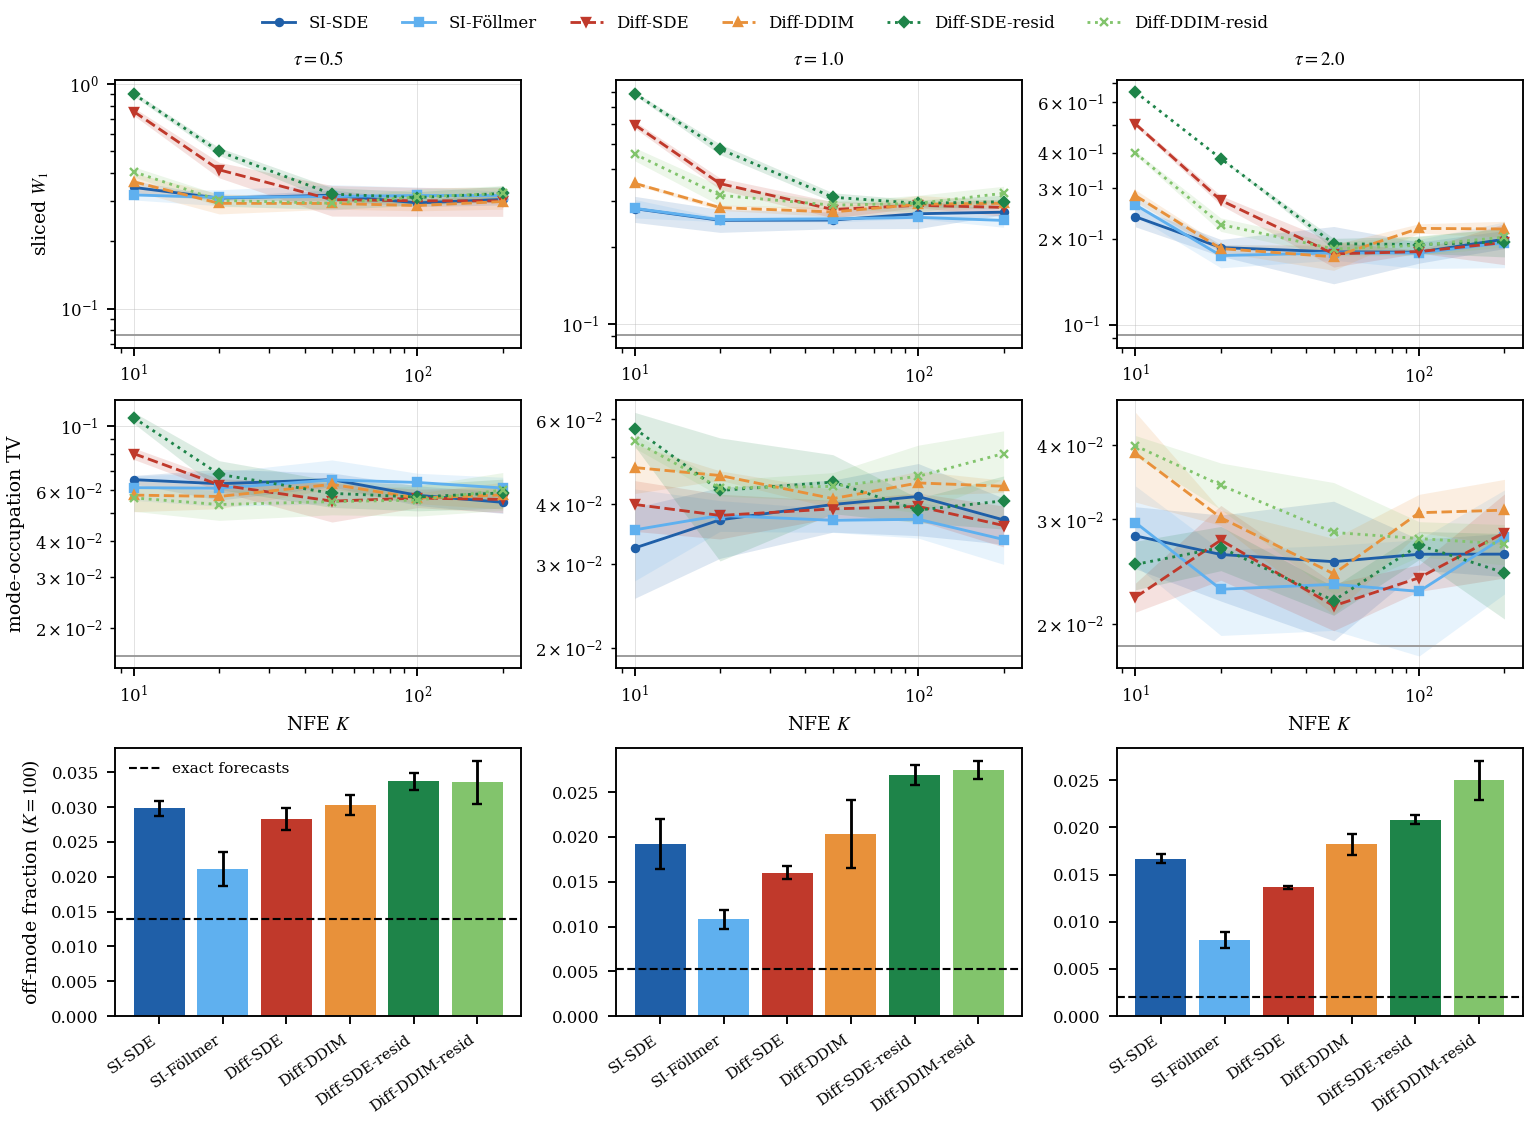
\includegraphics[width=\linewidth]{figures/fig_gmm_metrics.png}
    \caption{Forecasting the five-mode Gaussian-mixture jump-diffusion of \cite{chen2024forecasting}
at lags $\tau\in\{0.5,1,2\}$ (columns). All models share one MLP ($3\times128$, SiLU) trained with
Adam for 15k steps on $10^5$ stationary pairs; every sampler uses $K$ network evaluations (NFE) on a
uniform time grid. SI-SDE and SI-F\"ollmer sample the same learned interpolant drift from $X_0=x_0$
with noise $\sigma_s$ or the F\"ollmer coefficient $g^{\mathrm F}_s$; Diff-SDE and Diff-DDIM sample a
VP conditional diffusion model of $x_1$ from Gaussian noise with the reverse SDE or DDIM; the
\emph{-resid} variants model the normalized increment $(x_1-x_0)/c$. Forecasts (2{,}000 per initial
condition) are compared with $2\times10^4$ simulated paths from four initial conditions: a mode centre,
between two modes, near the origin, and an outer tail. \textbf{Top:} sliced $W_1$ distance.
\textbf{Middle:} total-variation error in the probability of landing in each mode (nearest of five
angular sectors). Curves are means over initial conditions; bands show $\pm1$ s.d.\ over 3 seeds; gray
lines are the Monte Carlo floor, i.e.\ the score of exact samples of the same size. \textbf{Bottom:}
fraction of forecasts at $K=100$ lying between modes; dashed line: exact forecasts; error bars: $\pm1$ s.d.\
over seeds.}
\label{fig1}
\end{figure}

\subsection{Mixed 2D Stochastic Navier-Stokes and Burger}
We follow the codebase of \cite{chen2024forecasting} which uses a pseudo-spectral solver with Euler-Maruyama time stepping (we use $200$ steps) to solve the PDE. We look at the 2D viscous Burgers equation of the form $\phi_t+\tfrac12|\nabla\phi|^2=\nu\Delta\phi+F$ with $u=\nabla\phi$ and $\nu=0.05$.
Each system has two trajectories of $100$ frames on a $256\times256$ grid. For Burgers, we replace $\omega$ with the divergence $\nabla\cdot u.$ In loading the data, each is downsampled to $128\times 128$ and $\omega_t$ is reduced to $64\times 64.$

Models are trained on frames $0$ to $79$ of each trajectory. Evaluation is done on frames $84, 90$ and $96.$ All models are trained with AdamW with a learning rate $\ell = 2\times 10^{-4}$ and a batch size of $8$.

For NS, we consider the random forcing
\begin{equation}
\label{eq:noise_construction}
\begin{aligned}
    \eta_{NS}(t,x,y) = &\big( W_1 (t)  \sin (6x) +  W_2 (t) \cos (7x) + W_3 (t) \sin (5(x+y)) + W_4 (t) \cos (8(x+y)) \big) \\
    & + \big( W_5 (t)  \cos (6x) +  W_6 (t) \sin (7x) + W_7 (t) \cos (5(x+y)) + W_8 (t) \sin (8(x+y)) \big),
\end{aligned}
\end{equation}
with $\nu=10^{-3},\alpha=0.1,\varepsilon=1$ and $W_i(t),1\le i\le 8$ are independent Wiener processes.
For Burger, we consider the random forcing
\begin{equation}
\label{eq:noise_construction_burgers}
\begin{aligned}
    \eta_B(t,x,y) = &\big( W_1 (t)  \sin (x) +  W_2 (t) \cos (x) + W_3 (t) \sin (y) + W_4 (t) \cos (y) \big) \\
    & + \big( W_5 (t)  \sin (x+y) +  W_6 (t) \cos (x+y) + W_7 (t) \sin (x-y + W_8 (t) \cos (x-y) \big).
\end{aligned}
\end{equation}

We create four datasets. One has purely NS data, one with purely Burger data, and two with a mixture of the data. We compare these with a deterministic approach trained using a UNet architecture $\hat\omega_{t+\tau}=f(\omega_t;\theta)$ trained using Mean Squared Error (MSE) loss function $\mathbb E\|\hat\omega_{t+\tau}-\omega_{t+\tau}\|^2$ with $\tau=1.$ This comparison is done using the estimated mean and std $\hat m, \hat \sigma$
\[
\text{err(mean)}=\frac{\|\hat m-m\|_{L^2}}{\|m\|_{L^2}},\quad\text{err(std)}=\frac{\|\hat\sigma-\sigma\|_{L^2}}{\|\sigma\|_{L^2}}.
\]

Let $\hat\omega$ be the Fourier coefficients of $\omega$. We define the enstrophy of the vorticity field $\omega$ as
\[
\text{Enstrophy}(k)=\sum_{k\leq |m|\leq k+1}|\hat\omega(m)|^2.
\]

\begin{figure}[t]
  \centering
  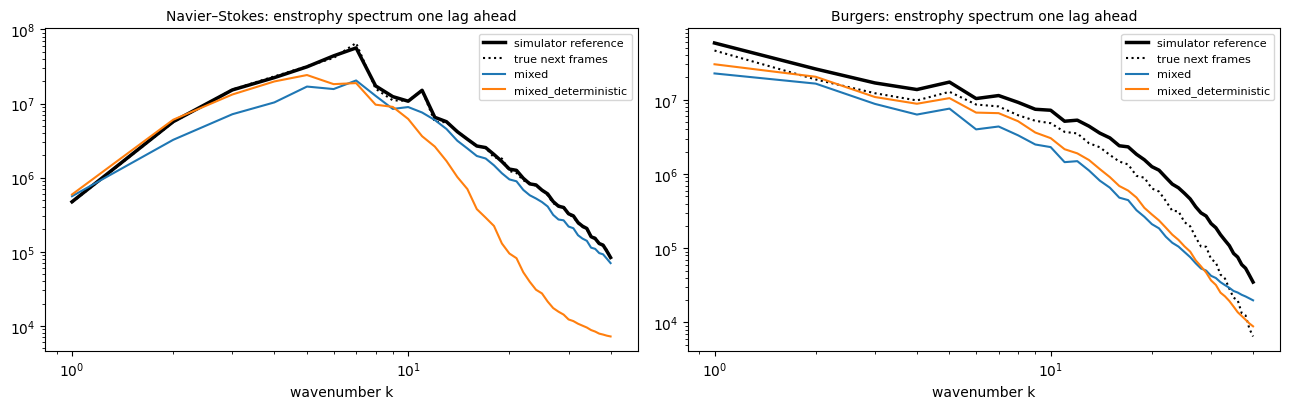
\includegraphics[width=\linewidth]{figures/enstrophy_mixed2.png}\\[4pt]
  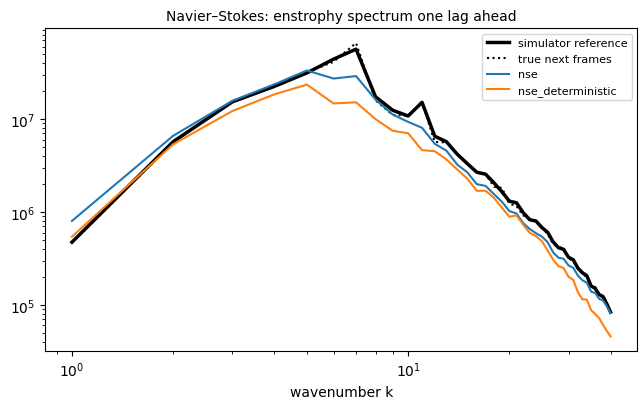
\includegraphics[width=0.49\linewidth]{figures/enstrophy_NSE.png}\hfill
  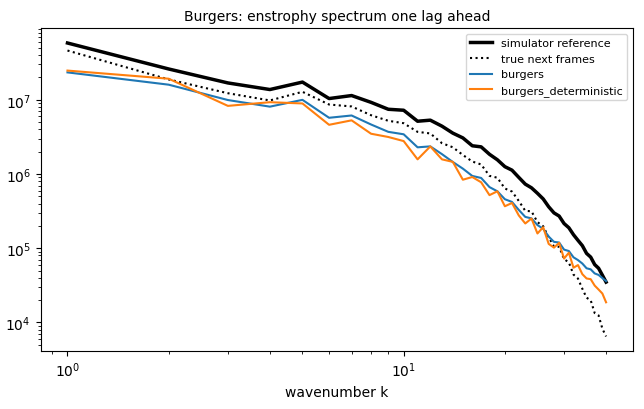
\includegraphics[width=0.49\linewidth]{figures/enstrophy_burger.png}
  \caption{The enstrophy spectra one lag agead ($\tau=1$) with interpolants $\alpha_s=1-s$, $\beta_s=s^2$, $\sigma_s=1-s$ and chosen so the diffusion term is $\sigma_sdW_s.$ Each is compared to the ground truth and a deterministic version. Over $6$ $\omega_t$ and $16$ independent ensembles of the forecast results $\hat\omega_{t+\tau}$ are averaged over to create the spectrum.
  \textbf{Top:} The enstrophy spectra of the model using a dataset with a 50:50 mixture of NSE and Burgers data.
  \textbf{Bottom:} On the left, the enstropy spectrum of the model trained on only NSE and on the right, the enstropy spectrum of the model trained on only Burger's equation.
  Generally, the performance of the mixed dataset is worse than that of the homogeneous datasets, especially around peaks.}
  \label{fig:enstrophy}
\end{figure}

\begin{table*}[ht]
  \centering
  \small
  \setlength{\tabcolsep}{4pt}
  \caption{Comparisons between the SDE approach and deterministic approach across the different datasets are shown of the short-time and long-time relative accuracy and the long-time of enstrophy. For the long-time row, the models are iterated for $20$ lags $\tau=1$ from $6$ held-out starts. The SDE model for Navier-Stokes does worse in the mixed sets, though Burgers performs slightly better with a 50:50 mixture.}
  \label{tab:errors}
  \begin{tabular}{@{}lcccccc@{}}
    \toprule
    & \multicolumn{2}{c}{Homogeneous} & \multicolumn{2}{c}{Mixed 90:10} & \multicolumn{2}{c}{Mixed 50:50} \\
    \cmidrule(lr){2-3} \cmidrule(lr){4-5} \cmidrule(l){6-7}
    Relative error & SDE & Det. & SDE & Det. & SDE & Det. \\
    \midrule
    \multicolumn{7}{@{}l}{\textit{Navier--Stokes}} \\
    Short-time $L^2$ error of mean & 6.2e-1 & 6.9e-1 & 6.5e-1 & 6.9e-1 & 7.7e-1 & 6.9e-1 \\
    Short-time $L^2$ error of std & 3.5e-1 & N/A & 6.3e-1 & N/A & 3.0e-1 & N/A \\
    Long-time error of avg.\ total enstrophy & 3.6e2\, & 6.7e-1\, & 6.1e0\,
      & 7.0e-1\, & 4.3e-1\, & 6.3e-1\, \\
    \midrule
    \multicolumn{7}{@{}l}{\textit{Burgers}} \\
    Short-time $L^2$ error of mean & 9.9e-1 & 1.3e0 & 1.5e0 & 9.7e-1 & 8.8e-1 & 1.1e0 \\
    Short-time $L^2$ error of std & 6.3e-1 & N/A & 7.5e-1 & N/A & 5.8e-1 & N/A \\
    Long-time error of avg.\ total enstrophy & 8.6e-1\, & 7.2e-1\, & 4.4e0\,
      & 8.6e-1\, & 1.8e-1\,& 8.3e-1\, \\
    \bottomrule
  \end{tabular}
\end{table*}

%%%%%%%%%%%%%%%%%%%%%%%%%%%%%%%%%%%%%%%%%%%%%%%%%%%%%%%%%%%%

\newpage
\section{CPU Smoke-Test Comparison for Continual Learning}
\label{app:cl-smoke}
To quickly compare continual-learning strategies before committing to the full
benchmark, we ran a representative AdvDiff1D smoke test on CPU. The smoke test
used two stream experiences, 16 snapshots per simulation, context length 3,
rollout length 2, one training epoch, batch size 32, and seed 123. All methods
used the same randomly initialized FNO1D model and were evaluated on the same
held-out stream. These results are diagnostic only and are not final benchmark
results.

\begin{figure}[t]
  \centering
  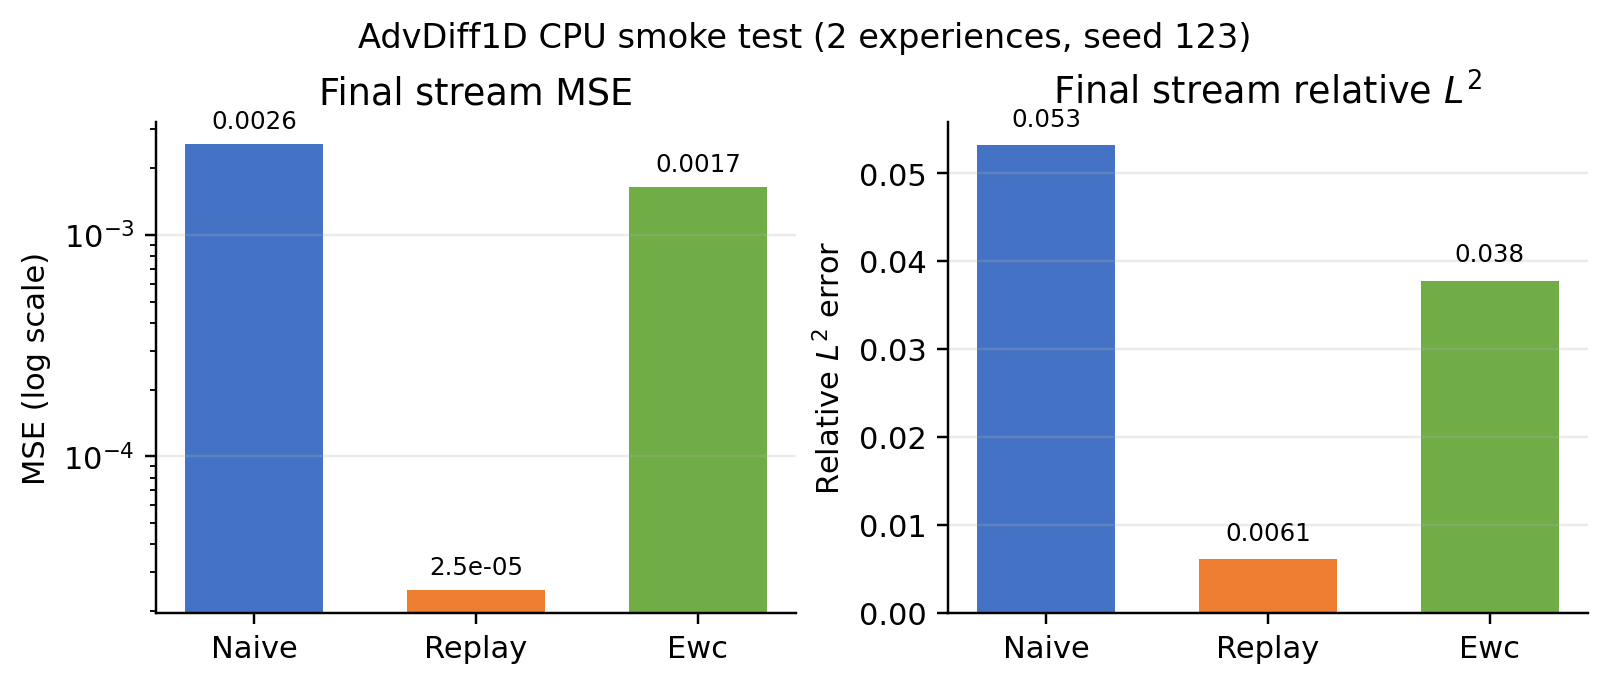
\includegraphics[width=0.92\linewidth]{figures/cl_smoke_method_comparison.png}
  \caption{Comparison on the AdvDiff1D stream. Lower
  values are better. Replay achieves the lowest final stream MSE and relative
  $L^2$ error in this fast diagnostic run.}
  \label{fig:cl-smoke-comparison}
\end{figure}

\begin{figure}[t]
  \centering
  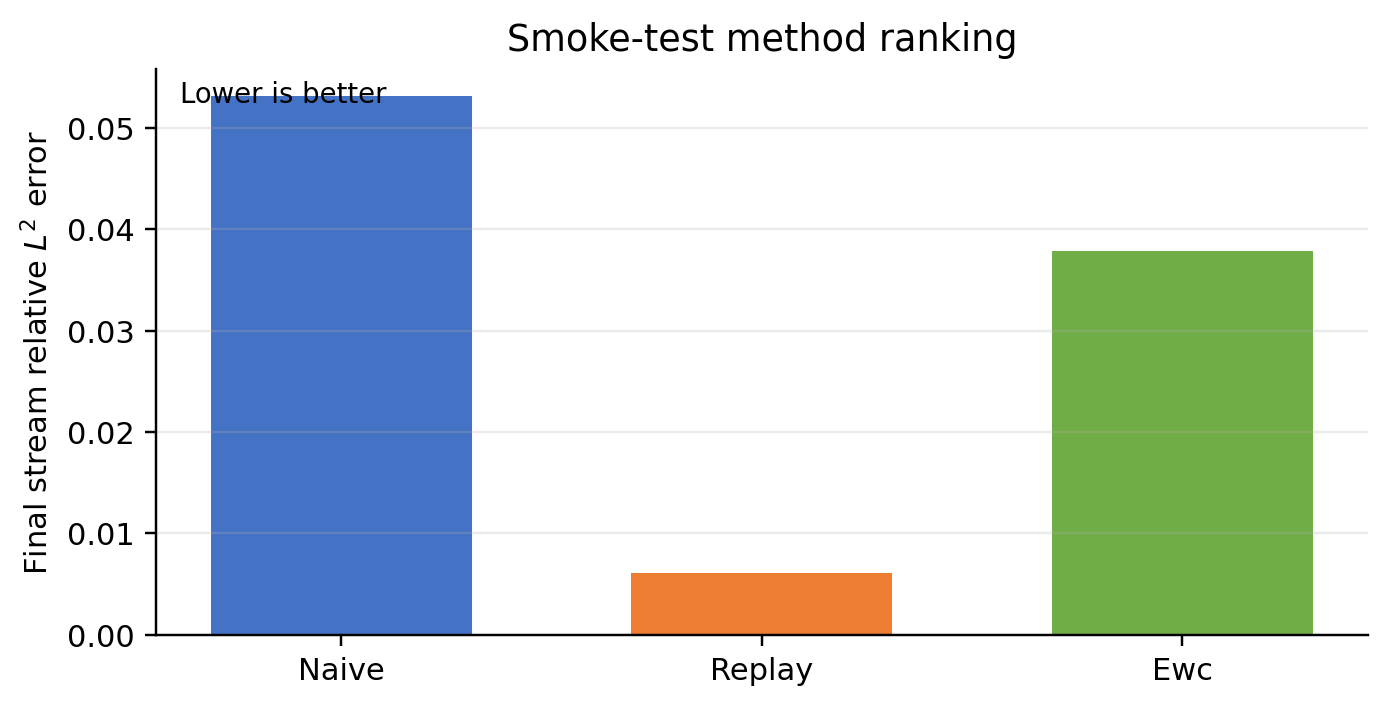
\includegraphics[width=0.72\linewidth]{figures/cl_smoke_relative_l2.png}
  \caption{Final stream relative $L^2$ error for the three smoke-test methods.}
  \label{fig:cl-smoke-relative-l2}
\end{figure}

Table~\ref{tab:cl-smoke} reports the final metrics. The complete reduced
configuration and reproducible runner are maintained with the experiment
artifacts; the smoke-test outputs are kept separate from the final benchmark
outputs.

\begin{table}[t]
  \centering
  \small
  \caption{Final metrics from the AdvDiff1D CPU smoke test.}
  \label{tab:cl-smoke}
  \begin{tabular}{lcc}
    \toprule
    Method & Stream MSE & Relative $L^2$ \\
    \midrule
    Naive & 0.002567 & 0.05318 \\
    Replay & 0.0000248 & 0.00611 \\
    EWC & 0.001650 & 0.03780 \\
    \bottomrule
  \end{tabular}
\end{table}


\end{document}
